
\documentclass[11pt,oneside,a4paper,onecolumn]{article}                 % Font/Document setup.
\usepackage{graphicx,color,setspace,hyperref}                           % Includes packages for the LaTeX document.
\usepackage[left=1.5in,top=1.25in,bottom=1.25in,right=1.25in]{geometry} % Sets the proper margins.

\setlength{\parindent}{0pt} % Do not automatically indent the paragraphs.

\begin{document}
\pagenumbering{roman} % Start the page numbering with Roman numerals.

%%%%%%%%%%%%%%%%%%%%%%%%%%%%%%%%%%%%
%%% Begin Title Page
%%%%%%%%%%%%%%%%%%%%%%%%%%%%%%%%%%%%

\thispagestyle{empty} % Suppress the page number for this page.
\begin{center}
UNIVERSITY OF CALIFORNIA\\
\ \\
SANTA CRUZ\\
\ \\
{\bf DESIGN, BUILDING, AND TESTING OF SUPERball:\\ A TENSEGRITY ROBOT FOR SPACE EXPOLRATION}\\
{\bf with an emphasis in ROBOTICS \& CONTROLS}
\ \\
\ \\
A thesis submitted in partial satisfaction\\
of the requirements for the degree of\\
\ \\
DOCTOR OF PHILOSOPHY\\
\ \\
in\\
\ \\
COMPUTER ENGINEERING\\
\ \\
by\\
\ \\
{\bf Jonathan Bruce}\\
\ \\
March 2015\\
\ \\
\ \\
\ \\
\end{center}

{\addtolength{\leftskip}{76.2 mm} % Indents three inches == 76.2 mm.
The Thesis of Jonathan Bruce\\
is approved:\\
\ \\
\ \\
--------------------------------------------------\\
Professor X, Chair\\
\ \\
\ \\
--------------------------------------------------\\
Professor\\
\ \\
\ \\
--------------------------------------------------\\
Professor Z\\*

}
\ \\
\ \\
\ \\
\ \\
--------------------------------------------------\\
Tyrus Miller\\
Vice Provost and Dean of Graduate Studies

\pagebreak[4]

%%%%%%%%%%%%%%%%%%%%%%%%%%%%%%%%%%%%
%%% End Title Page
%%%%%%%%%%%%%%%%%%%%%%%%%%%%%%%%%%%%

%%%%%%%%%%%%%%%%%%%%%%%%%%%%%%%%%%%%
%%% Begin Copyright Page
%%%%%%%%%%%%%%%%%%%%%%%%%%%%%%%%%%%%

\thispagestyle{empty} % Suppress the page number for this page.
\doublespacing
\begin{center}
\ \\
\ \\
\ \\
\ \\
\ \\
\ \\
\ \\
\ \\
\ \\
\ \\
\ \\
Copyright \copyright\ by\\
Sammy Slug\\
2011
\pagebreak[4]
\end{center}

%%%%%%%%%%%%%%%%%%%%%%%%%%%%%%%%%%%%
%%% End Copyright Page
%%%%%%%%%%%%%%%%%%%%%%%%%%%%%%%%%%%%

%%%%%%%%%%%%%%%%%%%%%%%%%%%%%%%%%%%%
%%% Begin Table of Contents Page
%%%%%%%%%%%%%%%%%%%%%%%%%%%%%%%%%%%%
\renewcommand\contentsname{Table of Contents} % This command changes the name of the autogenerated table of contents (next line) from "Contents" to "Table of Contents".
\tableofcontents % This command automatically generates the table of contents based on the sections in the document.
\pagebreak[4]

%%%%%%%%%%%%%%%%%%%%%%%%%%%%%%%%%%%%
%%% End Table of Contents Page
%%%%%%%%%%%%%%%%%%%%%%%%%%%%%%%%%%%%

%%%%%%%%%%%%%%%%%%%%%%%%%%%%%%%%%%%%
%%% Begin List of Figures Page
%%%%%%%%%%%%%%%%%%%%%%%%%%%%%%%%%%%%

\phantomsection % Create a phantom section such that the 'List of Figures' may be properly added to the table of contents.
\addcontentsline{toc}{section}{List of Figures} % Add this section, 'List of Figures', to the table of contents.
\listoffigures % This command automatically generates the list of figures based on the figures in the document.
\pagebreak[4]

%%%%%%%%%%%%%%%%%%%%%%%%%%%%%%%%%%%%
%%% End List of Figures Page
%%%%%%%%%%%%%%%%%%%%%%%%%%%%%%%%%%%%

%%%%%%%%%%%%%%%%%%%%%%%%%%%%%%%%%%%%
%%% Begin List of Tables Page
%%%%%%%%%%%%%%%%%%%%%%%%%%%%%%%%%%%%

\phantomsection % Create a phantom section such that the 'List of Tables' may be properly added to the table of contents.
\addcontentsline{toc}{section}{List of Tables} % Add this section, 'List of Tables', to the table of contents.
\listoftables % This command automatically generates the list of tables based on tables in the document.
\pagebreak[4]

%%%%%%%%%%%%%%%%%%%%%%%%%%%%%%%%%%%%
%%% End List of Tables Page
%%%%%%%%%%%%%%%%%%%%%%%%%%%%%%%%%%%%

%%%%%%%%%%%%%%%%%%%%%%%%%%%%%%%%%%%%
%%% Begin Abstract Page
%%%%%%%%%%%%%%%%%%%%%%%%%%%%%%%%%%%%
\thispagestyle{empty} % Suppress the page number for this page.
\phantomsection % Create a phantom section such that the 'Abstract' may be properly added to the table of contents.
\addcontentsline{toc}{section}{Abstract} % Add this section, 'Abstract', to the table of contents.
\begin{center}
{\bf Abstract}\\
\ \\
Investigation Into Why LaTeX Templates Don't Already Exist At An Engineering School\\
by\\
Sammy Slug\\
\end{center}
1. State the problem briefly.\\
2. Describe the methodology.\\
3. Summarize the findings.\\
ProQuest recommends that the Abstract be no longer than 350 words, as it may be posted to sites with limited file size


\pagebreak[4]

%%%%%%%%%%%%%%%%%%%%%%%%%%%%%%%%%%%%
%%% End Abstract Page
%%%%%%%%%%%%%%%%%%%%%%%%%%%%%%%%%%%%

%%%%%%%%%%%%%%%%%%%%%%%%%%%%%%%%%%%%
%%% Begin Dedication Page
%%%%%%%%%%%%%%%%%%%%%%%%%%%%%%%%%%%%

\phantomsection % Create a phantom section such that the 'Dedication' may be properly added to the table of contents.
\addcontentsline{toc}{section}{Dedication} % Add this section, 'Dedication', to the table of contents.

DEDICATION!

\pagebreak[4]

%%%%%%%%%%%%%%%%%%%%%%%%%%%%%%%%%%%%
%%% End Dedication Page
%%%%%%%%%%%%%%%%%%%%%%%%%%%%%%%%%%%%

%%%%%%%%%%%%%%%%%%%%%%%%%%%%%%%%%%%%
%%% Begin Acknowledgments Page
%%%%%%%%%%%%%%%%%%%%%%%%%%%%%%%%%%%%

\phantomsection % Create a phantom section such that the 'Acknowledgments' may be properly added to the table of contents.
\addcontentsline{toc}{section}{Acknowledgments} % Add this section, 'Acknowledgments', to the table of contents.

ACKNOWLEDGMENTS!

\pagebreak[4]

%%%%%%%%%%%%%%%%%%%%%%%%%%%%%%%%%%%%
%%% End Acknowledgments Page
%%%%%%%%%%%%%%%%%%%%%%%%%%%%%%%%%%%%

\pagenumbering{arabic} % Change the page numbering back to arabic numerals.
\section{Introduction}
Introduction information will go in here...

\section{Related Work}
Related work information will go in here...

\section{Method}
Method information will go in here...
  
\section{Experiments}
Experiments information will go in here...
  
\section{Results}
Results information will go in here...
  
\section{Discussion}
Discussion information will go in here...\cite{yan2007determining}\\ % One citation used to show how to use.
\pagebreak[4]

\section{Test Figure/Table}
Below are a test figure and a test table to show usage, and that they actually populate the automatically generated lists at the beginning of the document.

\begin{figure}[h!] % Create and insert the figure into the document.
  \centering
    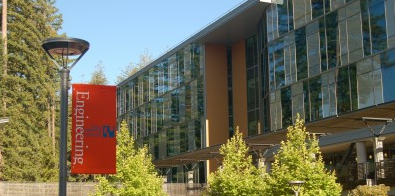
\includegraphics[width=0.5\textwidth]{./img/bsoe_outside.png} % Include the graphic in the specified location to the figure.
    \caption{Outside of the BSOE.}
\end{figure}

\begin{table}[h!] % Create a very simple table to show workingness.
  \begin{center}
    \begin{tabular}{| l c r |}
    \hline
    1 & 2 & 3 \\
    4 & 5 & 6 \\
    7 & 8 & 9 \\
    \hline
    \end{tabular}
  \end{center}
  \caption{A simple table.}
\end{table}


\phantomsection % Create a phantom section such that the 'Acknowledgments' may be properly added to the table of contents.
\addcontentsline{toc}{section}{References} % Add this section, 'References', to the table of contents.
\bibliographystyle{plain} 
\bibliography{Advancement_Doc_Jonathan_Bruce} % Create bibliography using the files in: "./".

\end{document}
